%%%%%%%%%%%%%%%%%%%%%%%%%%%%%%%%%%%%%%%%%%%%%%%%%%%%%%%%%%%%%%%%%%%%%%%%%%%%%%%
\subsection{Characteristics of Bees}
%%%%%%%%%%%%%%%%%%%%%%%%%%%%%%%%%%%%%%%%%%%%%%%%%%%%%%%%%%%%%%%%%%%%%%%%%%%%%%%
By inspecting the characteristics of each honey bee, concerning its degree~$k$, strength~$s$, local clustering coefficient~(lcc)~$c$, betweenness centrality~$C_B$ and closeness centrality~$C_C$, properties of the honey bee colony can be derived.



\paragraph{Low Hierarchical Structure}
The degree is normally distributed (a in figure~\ref{fig:n3-degreeStrLCC}).
Therefore most bees bee have the same high number of interaction partners.
The absence of hubs, a small number of highly connected bees, indicates a low hierarchical structure of the network.
Strength and lcc are also normally distributed (d and g in figure~\ref{fig:n3-degreeStrLCC}).
That also shows the absence of extreme values and confirms that bees are similar to each other regarding those properties.
Betweenness and closeness centrality (j and m in figure~\ref{fig:n3-degreeStrLCC}) also follow a normal distribution.
This leading to the assumption that no central or important bees exist.
All bees are similarly close to all other bees in the network, and every bee can reach any other bee with a few steps.
That also corresponds to the low average path length, and the small diameter of the network described in section~\ref{subsec:colony}.
The absence of bees with a high betweenness suggests that the colonies functionality is robust concerning the disappearance of single individuals.

\paragraph{Correlation of Local Measures and Detection Frequency}
Degree and detection frequency are positively correlated.
The higher the degree, the higher the detection frequency.


\paragraph{Tendency of Age Cohorts}
tendency for bimodality: betweeness, closeness, degree, strength\\
lcc tendency for beeing right skewed\\
old group > 45 days: low degree, strength, $C_B$ and $C_C$, but high lcc, not good connected to each other, less detected\\
rest < 45: high degree, strength, $C_B$, $C_C$, but low lcc, good connected to each other, high detection frequency\\
Figure~\ref{fig:n3-degree} shows a wide ranged bimodal degree distribution, with a border at about $0.4$. It indicates the presence of two groups.
The first group, which is much smaller than the second group, interacts on average with 20\% of the population, and the second with on average of 80\%, corresponding to almost the entire population.
The age-degree correlation plot shows that bees, that are older than 45 days do have a lower degree than younger bees ($< 45$ days).
Old bees, with a low detection frequency and a low number of interaction partners, could be foragers, because they spend much time outside the hive, and are therefore less often detected. Younger bees spend more time inside the hive. Therefore they have a higher detection frequency and more time to gather bees they interact with
Figure~\ref{fig:n3-strength} shows a wide range bimodal strength distribution. There is a first peak at the lowest value and a second peak at about $5000$. This also corresponds to two groups of bees. The first group of bees is older than 45 days has a very low strength and low detection frequency. The second group with an age younger than 45 days with a high strength.
A high strength can result from lots of neighbours with low edge weights or a few neighbores with high edge weight. The second is rather unlikeliy, looking at the edge weight distribution (figure~\ref{fig:edgeWdist}). The strength distibution is very similar to the degree distribution.
Old bees, which might be foragers are charcterized by a low degree, correspondingly low strength but by a higher lcc compared to younger bees. A high lcc indicates a high connection between the neighbours of a foragers. Young bees have a low lcc, meaning that its neighbours (also foragers) are not connected to each other.
A right skewed local clustering coefficient distribution is shown in figure~\ref{fign3-lcc}, with a peak at $0.75$.
Here it is the other way around, a high value corresponds to a low detection frequency and therefore to an older bees, again over 45 days old.



\begin{figure}[!htb]
	\centering
	\begin{subfigure}[b]{1.0\textwidth}
	\centering
	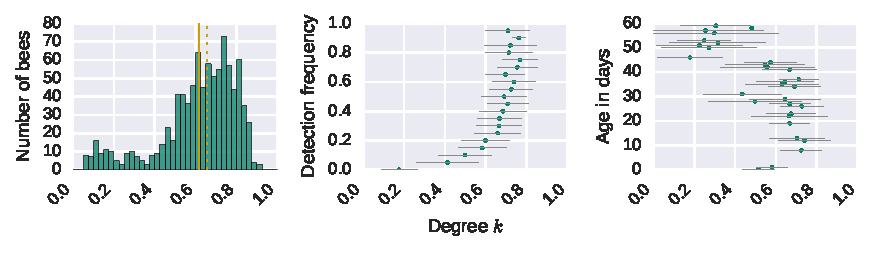
\includegraphics[width=1.0\textwidth]{Figures/n3-stat-degreeAgeDetF.pdf}
	%\caption[Degree]{\textbf{Degree}}
	%\label{fig:n3-degree}
	\end{subfigure}
	\begin{subfigure}[b]{1.0\textwidth}
	\centering
	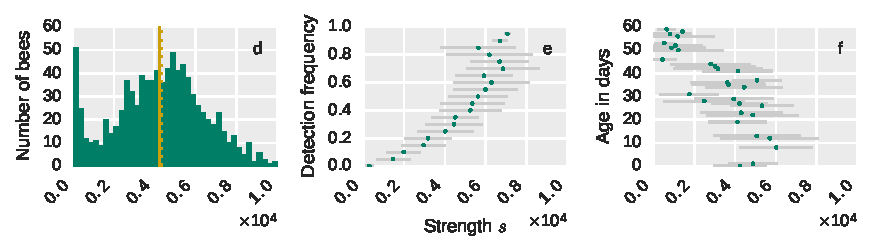
\includegraphics[width=1.0\textwidth]{Figures/n3-stat-strengthAgeDetF.pdf}
	%\caption[Strength]{\textbf{Strength}}
	%\label{fig:n3-strength}
	\end{subfigure}
	\begin{subfigure}[b]{1.0\textwidth}
	\centering
	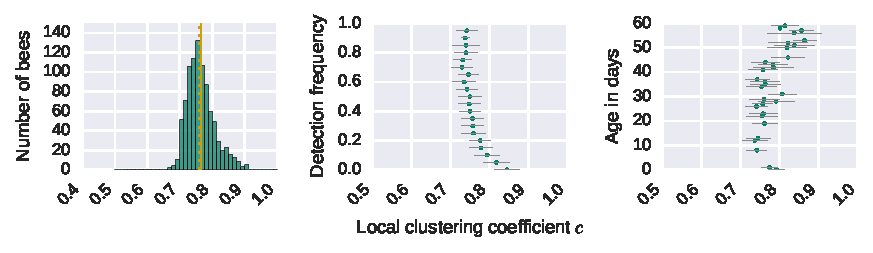
\includegraphics[width=1.0\textwidth]{Figures/n3-stat-lccAgeDetF.pdf}
	%\caption[Local clustering coefficient]{\textbf{Local clustering coefficient}}
	%\label{fig:n3-lcc}
	\end{subfigure}
	\begin{subfigure}[b]{1.0\textwidth}
	\centering
	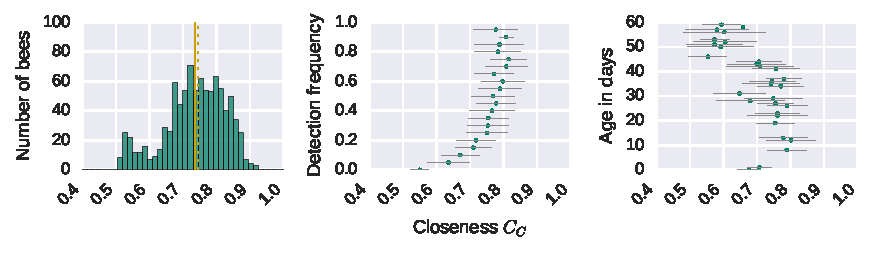
\includegraphics[width=1.0\textwidth]{Figures/n3-stat-closenessAgeDetF.pdf}
	%\caption[Closeness Centrality]{\textbf{Closeness Centrality}}
	%\label{fig:n3-closeness}
	\end{subfigure}
	\begin{subfigure}[b]{1.0\textwidth}
	\centering
	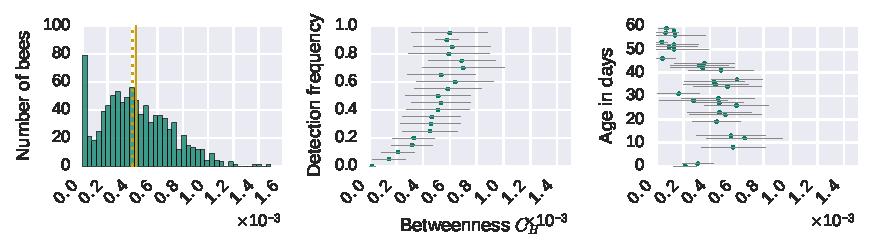
\includegraphics[width=1.0\textwidth]{Figures/n3-stat-betweenAgeDetF.pdf}
	%\caption[Betweeness Centrality]{\textbf{Betweeness Centrality}}
	%\label{fig:n3-between}
	\end{subfigure}
	\caption[Degree, strength and local clustering coefficient (LCC)]{\textbf{Degree, strength and local clustering coefficient (LCC) in relation to age and detection frequency} xxx}
	\label{fig:n3-degreeStrLCC}
\end{figure}